\documentclass{beamer}
\usepackage[spanish]{babel}
\usepackage[T1]{fontenc}
\usepackage[utf8]{inputenc}
\usepackage{lmodern}
\usepackage{amssymb}
\usepackage{graphicx}
\usepackage{amsthm}
\usepackage{amsmath}
\usepackage{mathtools}
\usepackage{xspace}
\usepackage{adjustbox}
\usepackage{caption}


\captionsetup[table]{labelformat=empty}% redefines the caption setup of the figures environment in the beamer class.

\uselanguage{spanish}
\languagepath{spanish}


\def\tituloTesis{Métricas de mimetización acústico-prosódica en hablantes y su relación con rasgos sociales de diálogos}

\title[Métricas de mimetización]{\tituloTesis}
\author[Juan Manuel Pérez]{Juan Manuel Pérez \and Agustín Gravano \and Ramiro H. Gálvez}
\institute[]{Departamento de Computación, FCEyN, UBA}
\date{Concurso de Tesis 2016}
\usetheme{Madrid}


\DeclareMathOperator*{\argmax}{arg\,max}

\begin{document}

\beamertemplatenavigationsymbolsempty



\frame{\titlepage}

\newcommand{\absentrainment} {\emph{absolute entrainment}\xspace}
\newcommand{\fwentrainment}[1] {\mathcal{E}_{#1}}

\newcommand{\entrainment} {\emph{entrainment}\xspace}
\newcommand{\disentrainment} {\emph{disentrainment}\xspace}

\newcommand{\TAMA} {\emph{TAMA}\xspace}
%%% Variables A/P
\newcommand{\ENGMAX} {ENG\_MAX\xspace}
\newcommand{\ENGMEAN} {ENG\_MEAN\xspace}
\newcommand{\FOMAX} {F0\_MAX\xspace}
\newcommand{\FOMEAN} {F0\_MEAN\xspace}
\newcommand{\TOTFRAMES} {VCD2TOT\_FRAMES\xspace}
\newcommand{\NOISETOHARMONICS} {NOISE\_TO\_HARMONICS\_RATIO\xspace}
\newcommand{\SYLCOUNT} {SYLLABES\_COUNT\xspace}
\newcommand{\SYLAVG} {SYLLABES\_COUNT\xspace}
\newcommand{\LOCALSHIMMER} {SOUND\_VOICED\_LOCAL\_SHIMMER\xspace}
\newcommand{\PHONCOUNT} {PHONEMES\_COUNT\xspace}
\newcommand{\PHONAVG} {PHONEMES\_AVERAGE\xspace}


%%% variables sociales

\newcommand{\socialvariable}[1] {\emph{#1}}
\newcommand{\svcontributes} {\socialvariable{contributes-to-completion}}
\newcommand{\svclear} {\socialvariable{making-self-clear}}
\newcommand{\svengaged} {\socialvariable{engaged-with-game}}
\newcommand{\svplanning} {\socialvariable{planning-what-to-say}}
\newcommand{\svencourages} {\socialvariable{gives-encouragement}}
\newcommand{\svdifficult} {\socialvariable{difficult-for-partner-to-speak}}
\newcommand{\svbored} {\socialvariable{bored-with-game}}
\newcommand{\svdislikes} {\socialvariable{dislikes-partner}}

%%% Regresión and stuff
\newcommand{\estslope} {\widehat{\beta_2}}
\newcommand{\myhighlight} {\rowcolor[gray]{.75}}

%%% Nota
\newcommand{\nota}[1]{\todo{#1}}



Los sistemas de diálogo humano-computadora son cada vez más frecuentes, y sus aplicaciones comprenden una amplia gama de rubros: desde aplicaciones móviles, motores de búsqueda, juegos o tecnologías de asistencia para ancianos y discapacitados. Si bien es cierto que estos sistemas logran captar la dimensión lingüística de la comunicación humana, tienen un déficit importante a la hora de procesar y transmitir el aspecto superestructural de la comunicación oral, que radica en el intercambio de afecto, emociones, actitudes y otras intenciones de los participantes. Este problema puede verse en cualquier sistema que interactúe sintetizando lenguaje humano: por ejemplo, las aplicaciones telefónicas que atienden automáticamente a sus clientes \cite{pieraccini2005,raux2006}. Stanley Kubrick y Arthur C. Clarke predijeron esto a la perfección, cuando en ``2001: Una Odisea en el Espacio''(1968) dotaron a \emph{HAL} de una voz monótona y robótica, casi lobotomizada. Otro problema grave que sufren estos sistemas humano-computadora es que asumen que sus interacciones de ``a turnos'', cuando las conversaciones entre humanos suelen distar bastante de ese modelo.

Dentro de las cualidades del lenguaje oral, una de las más distintivas es la \emph{prosodia}, qué es la dimensión que capta \emph{cómo} se dicen las cosas, en contraposición a \emph{qué} se está manifestando. Posee varias componentes acústico-prosódicas: por ejemplo, el tono o pitch, la intensidad o volumen, la calidad de la voz, la velocidad del habla y otras. Un manejo adecuado de estas componentes es lo que, hoy día, distingue una voz humana de una artificial. Esta carencia de habilidad sobre la prosodia conlleva cierta dificultad en la interacción con agentes conversaciones, que suelen ser calificados como ``mecánicos'' o ``extraños'' en su forma de comunicarse. \cite{raux2006,ward2005}

En pos de mejorar el entendimiento entre agentes conversacionales y sus usuarios, resulta de vital importancia poder entender y modelar las variaciones prosódicas de la comunicación oral. Esto se traduciría tanto en una mejor apreciación de lo que quiere comunicar el usuario, como en una mayor naturalidad de la voz sintetizada por el agente.

\subsection{Mimetización}

En la literatura de Psicología del Comportamiento se ha observado con frecuencia que, bajo ciertas condiciones, cuando una persona mantiene una conversación, ésta modifica su manera de actuar aproximándola a la de su interlocutor. En una reseña de este tema se describe a este fenómeno como una ``imitación no consciente de posturas, maneras, expresiones faciales y otros comportamientos del compañero interaccional'' \cite[p. 893]{CHAR1999}  y conjeturan que es más fuerte en individuos con empatía disposicional. En otras palabras, personas con predisposición a buscar la aceptación social modifican su comportamiento en forma más marcada para aproximarlo a sus interlocutores

Esta modificación del comportamiento ha sido observada también en la manera de hablar. Por ejemplo, los interlocutores adoptan las mismas formas léxicas para referirse a las cosas, negociando tácitamente descripciones compartidas, en especial para cosas que resulten poco familiares \cite{BRE1996}. Estudios más recientes sugieren que esto también es cierto para el uso de estructuras sintácticas \cite{REI2006}. Este fenómeno subconsciente es conocido como mimetización, alineamiento, adaptación o convergencia y también con el término inglés \entrainment. Se ha mostrado que juega un rol importante en la coordinación de diálogos, facilitando tanto la producción como la comprensión del habla en los seres humanos\cite{nenkova2008,gravano2015backward}. En nuestro caso, nos interesa principalmente el \entrainment de la prosodia.

\subsection{Midiendo la mimetización}

Muchos estudios han examinado la mimetización prosódica, listados en \cite{DEL2013}. Un número importante de ellos se han basado en la premisa de la mimetización como un fenómeno lineal, en el cual la convergencia ``va sucediendo'' a lo largo de la conversación \cite{burgoon1995interpersonal}. Estos estudios dividen las conversaciones en varias partes, y verifican que la diferencia absoluta entre los valores medios (de las variables \ap) y sus desviaciones se aproxime en las últimas partes de la interacción. Sin embargo, este enfoque de la mimetización niega su faceta dinámica: los interlocutores pueden estar inactivos y luego hablar, pueden pasar por varias etapas como escuchar, pensar, discutir un punto, etc. En \cite{levitan2011measuring} se reportó que éste es un fenómeno no sólamente lineal, sino también dinámico, donde los interlocutores van coincidiendo en el análisis por turnos.

Un problema común que surge a la hora de calcular estas métricas es el hecho de que las conversaciones no están alineadas en el tiempo, ni se dan en turnos de duración constante. Nos preguntamos entonces qué partes del diálogo de un hablante deberían compararse con qué otras partes de su par. Un enfoque de comparar interlocuciones uno a uno es demasiado simple y no captura situaciones de diálogo reales, mucho más dinámicas y con solapamiento casi constante.

Para atacar estos inconvenientes, utilizamos el método \TAMA(Time Aligned Moving Average) \cite{KOU2008}, que consiste en separar en ventanas de tiempo el diálogo, y promediar los valores de las variables prosódicas dentro de cada una. Este método es muy similar a aplicar un filtro de Promedio Móvil (Moving Average), lo que da el nombre a la técnica. Al separar el diálogo en ventanas de tiempo, podemos construir dos series de tiempo en base a cada interlocutor. Estas abstracciones son mucho más tratables que tener una secuencia de elocuciones de parte de cada hablante, y nos permiten efectuar análisis bien conocidos, uno de los cuáles nos permite construir una medida del \entrainment.

\subsection{Objetivo del estudio}

En el presente estudio, aplicamos la técnica de \TAMA para definir dos métricas de \entrainment. Utilizamos un corpus de diálogo entre dos participantes angloparlantes, quienes interactúan mediante un juego a través de computadoras. El corpus ha sido anotado manualmente con variables que describen la percepción social de la conversación; por ejemplo: ¿el sujeto parece comprometido con el juego? ¿al sujeto no le agrada su compañero?

Luego, veremos si existe, para cada una de las variables \ap,  alguna relación significante entre las métricas definidas y las percepciones sociales sobre las conversaciones. Uno esperaría que valores altos de nuestras métricas del \entrainment se relacionen con valores altos de variables sociales positivas, tales como mostrarse colaborativo o compenetrado en la tarea. 



\section{Materiales y Métodos}
En esta sección describiremos tanto el corpus utilizado en el estudio, como así también las modificaciones que efectuamos sobre el método TAMA.

\section{Columbia Game Corpus}

\newcommand{\objectgame} {\emph{Juego de objetos}}


Empleamos el Columbia Game Corpus  \cite{GRAV2009} consiste en doce conversaciones diádicas (i.e., con dos participantes) entre trece personas angloparlantes distintas. Todos los participantes reportaron hablar Inglés Americano Estándar, y no tener problemas de audición. La edad de los participantes se encuentra en el rango de los 20 a 50 años.

Las grabaciones se hicieron en 44 kHz, 16 bits con un canal separado para cada hablante; luego fueron guardadas en 16 kHz para el presente estudio. Cada sesión duró aproximadamente 45 minutos, totalizando 9 horas de
diálogos, 70.259 palabras (2.037 únicas) para todo el cuerpo de datos.

En cada sesión, se sentó a dos participantes (quienes no se conocían previamente) en una cabina profesional de grabación, cara a cara a ambos lados de una mesa, y con una cortina opaca colgando entre ellos para evitar la comunicación visual. Los participantes contaron con sendas computadoras portátiles conectadas entre sí, en las cuales jugaron una serie de juegos simples que requerían de comunicación verbal. El primero de ellos, un juego de cartas que no consideramos en el presente estudio por tratarse esencialmente de monólogos o diálogos con poca interacción. Luego de esto, pasaron al juego que analizamos, denominado `juego de objetos'.

\subsection{Juego de Objetos}

En el juego de objetos, la pantalla de cada jugador mostró un tablero con varios objetos, entre 5 y 7, como se ve en la figura \ref{objects_game}.
Para uno de los jugadores (el Descriptor) el objeto \emph{Objetivo} aparecía en una posición aleatoria entre otros objetos. Para el otro jugador, a quien llamaremos el Seguidor, el objetivo aparecía en la parte baja de la pantalla. Entonces, al Descriptor se le encargaba describir la posición del Objetivo de manera que el Seguidor pudiera mover su representación del objeto a la misma posición en su pantalla. Luego de una negociación entre ambos jugadores para decidir la mejor posición del objeto, se les asignó a los jugadores una puntuación entre 1 y 100 puntos de acuerdo a qué tan acertado fue el posicionamiento del objetivo por parte del Seguidor.

\begin{figure}
\centering
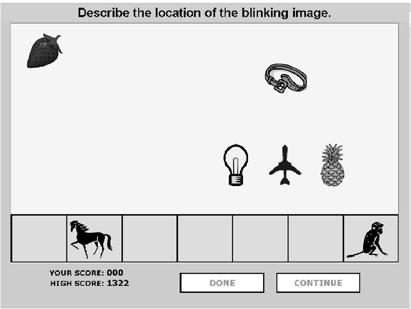
\includegraphics[scale=0.5]{images/columbia_games.jpg}
\caption{Juego de objetos del Columbia Games}
\label{objects_game}
\end{figure}


Cada sesión consistió de 14 tareas como ésta, cambiando los objetos y sus ubicaciones. En las primeras cuatro tareas, uno de los sujetos tomó el papel del Descriptor; en los siguientes cuatro invirtieron roles, y en las finales seis fueron alternando los roles de Descriptor y Seguidor.

\subsection{Anotaciones sobre comportamiento social}

Varios aspectos del comportamiento de los jugadores durante los juegos de objetos fueron anotados mediante la herramienta de crowdsourcing \emph{Amazon Mechanical Turk}. Cada anotador escuchó el audio correspondiente a una tarea del juego y tuvo que responder a varias preguntas sobre cada uno de los sujetos, entre las que se encuentran:

\begin{itemize}
  \item ¿el sujeto parece comprometido con el juego?
  \item ¿el sujeto dirige la conversación?
  \item ¿el sujeto contribuye para el éxito del equipo?
  \item ¿el sujeto alienta a su compañero?
  \item ¿el sujeto se expresa correctamente?
  \item ¿al sujeto no le agrada su compañero?
  \item ¿el sujeto le hace difícil hablar a su compañero?
  \item ¿el sujeto intenta acaparar la conversación?
\end{itemize}

\noindent Cada uno de estos audios fue puntuado por cinco anotadores, que respondieron por sí o por no para cada una de las preguntas. El puntaje que recibe cada una de las preguntas (a las cuales llamaremos a partir de ahora \emph{variables sociales}) consiste en la cantidad de respuestas afirmativas que recibió, teniendo un rango de 0 a 5. Por ejemplo, una tarea dada podría tener puntaje 3 para la variable social `el sujeto A se expresa correctamente' o puntaje 5 para la variable `el sujeto B dirige la conversación'.

\subsection{Extracción de variables acústico/prosódicas}

La herramienta \emph{Praat} fue utilizada para extraer automáticamente las variables \ap del corpus. Las variables que medimos fueron el tono, la intensidad, la proporción de vocalizaciones, jitter, shimmer, cantidad de sílabas, cantidad de fonemas, y la proporción de ruido sobre armónicos. Estos atributos fueron medidos en cada uno de los segmentos de habla del corpus.

Repasemos algunos conceptos que necesitamos para definir las variables acústicas.

\begin{itemize}
  \item \emph{f0} refiere a la frecuencia fundamental de una onda, que es el recíproco del período de ésta. El \emph{tono} o \emph{pitch} es la percepción que tenemos de la frecuencia fundamental, que nos marca cuán agudos o graves son los sonidos.
  \item \emph{Intensity} refiere al volumen o intensidad de la onda. Ésta mide la amplitud de la onda, y es la percepción de cuán fuerte es el sonido.
  \item \emph{jitter y shimmer} se refieren, en un intervalo de tiempo, a los desplazamientos de la onda de la verdadera periodicidad y de la amplitud, respectivamente. Están asociadas con la percepción de la calidad de la voz.
  \item Un \emph{fonema} es la articulación simple de sonidos del habla, tanto de vocales como de consonantes. Ejemplos de fonemas son los sonidos de las letras u, a, s, k en español.
  \item El \emph{noise-to-harmonics ratio} (abreviado NHR) puede considerarse como una medida de calidad de la voz, que cuantifica la proporción de ruido que hay en ésta.
\end{itemize}


En la siguiente tabla resumimos estas features. Recordemos nuevamente que estas features son medidas en un intervalo de tiempo.

\begin{figure}[h!]
\centering
\resizebox{\textwidth}{!}{
\begin{tabular} {|c|c|}
  \hline
  Variable a/p & Descripción \\
  \hline
  \hline
  \FOMEAN & Valor medio de la frecuencia fundamental \\\hline
  \FOMAX  & Valor máximo de la frecuencia fundamental \\\hline
  \ENGMEAN & Valor medio de la intensidad \\\hline
  \ENGMAX & Valor máximo de la intensidad \\\hline
  \NOISETOHARMONICS & Noise-to-harmonics descripto anteriormente \\\hline
  \LOCALSHIMMER & Shimmer medido \\\hline
  \SYLAVG & Cantidad de sílabas por segundo \\\hline
  \PHONAVG & Cantidad de fonemas por segundo \\\hline
\end{tabular}
}
\end{figure}

\section{Modificaciones a TAMA}
\label{sec:tama_modifications}
Al método TAMA descripto en \ref{sec:ant_tama} le hemos aplicado algunas variaciones, que pasaremos a detallar.

En primer lugar, \cite{KOU2008.2} discute la disyuntiva de elegir un tamaño de ventana y step para el método: ventanas demasiado chicas pueden causar que no hayan segmentos de habla en ellas, mientras que un tamaño de ventana demasiado grande suavizaría en exceso la serie de tiempo. A colación de esto, dicho trabajo menciona dos posibles soluciones para el problema de los puntos faltantes: interpolar (también mencionado en \cite{DEL2013}) o repetir el punto anterior de la serie.

Estos enfoques, sin embargo, pueden dar lugar a valores de \entrainment artificialmente altos por la construcción misma de la serie, ya que nos generaría puntos correlacionados fuertemente entre sí en cada una de las series de los hablantes. Por otro lado, descartar aquellas conversaciones que tengan puntos faltantes puede ser demasiado restrictivo y eliminar de nuestro corpus una gran cantidad de datos valiosos. Teniendo estas cosas en mente, decidimos aceptar series de tiempo con datos faltantes, que pueden ser producto de ventanas sin segmentos de habla o con algunos demasiado pequeños que imposibiliten la medición de las variables \ap: por ejemplo interjecciones o backchanneling (\emph{uh-huh} o \emph{hmmm} en inglés).

\section{Selección de Ventana}

En \cite{KOU2009} se menciona una elección de \emph{frame step} y \emph{frame length} de 10s y 20s respectivamente. En el caso de nuestro corpus, quisimos buscar los parámetros que mejor se ajustaban a éste, manteniendo la superposición del 50\% entre ventanas sucesivas. Con lo que nos queda que $FL = 2 * FS$

¿Qué queremos optimizar? La métrica que elegimos para ésto es encontrar un balance entre un frame no tan grande (para no suavizar en exceso la curva) y que nos reduzca considerablemente la cantidad de indefiniciones; es decir, aquellas ventanas que tomamos en un interlocutor que no tienen ninguna interacción de su parte. Para ver ésto, graficamos la cantidad de indefiniciones en función del step tomado.

\begin{figure}
\centering
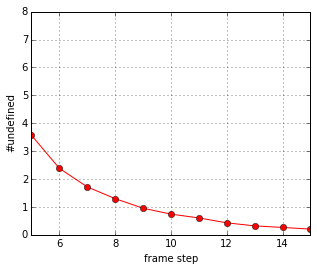
\includegraphics[width=10cm]{images/window_selection.png}
\end{figure}



Dentro del rango de $FS \in \{5'',6'', \ldots ,15'' \}$, graficamos para cada sesión, tarea y cada interlocutor las curvas de indefiniciones. A su vez, para mayor claridad, graficamos una curva que promedie todas las tareas de una sesión.


Para tener una visión general de lo que ocurría en todas las sesiones, graficamos una curva promedio de todas las sesiones. En ésta puede observarse que hasta $8''-10''$ hay un fuerte descenso de las indefiniciones, que luego se atenúa. Dado que en general tenemos tareas cortas, preferimos tomar $8''$ como step, y $16''$ como largo de ventana.

OBS: podríamos cambiar ésto a un boxplot!

\begin{figure}
\centering
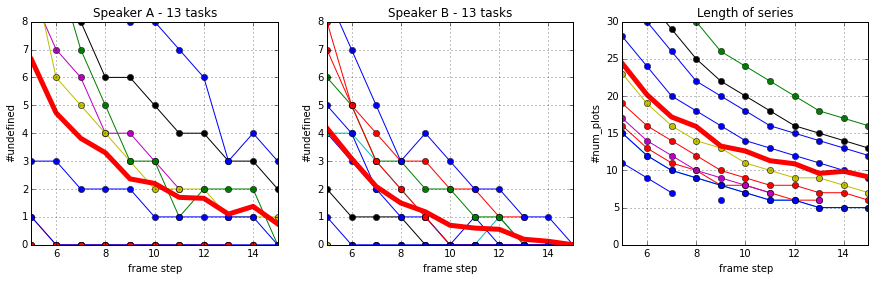
\includegraphics[height=5cm]{images/window_selection_for_session.png}
\end{figure}


\section{Time plots}
\label{sec:time_plots}
Usando la técnica descripta con las variaciones que consideramos en la anterior sección, generamos dos series de tiempo para cada tarea. Como antes mencionamos, la ventana elegida es de 16 segundos con un step de 8 segundos lo cual da un overlap del 50\%.

Dada una ventana, puede ocurrir que alguno de los interlocutores no haya hablado, o su interacción haya sido demasiado breve como para medir sus variables \ap. Como ya mencionamos en la sección \ref{sec:tama_modifications}, y a diferencia de \cite{KOU2008.2}, construimos las series sin ese punto, y sin interpolarlo tampoco.

De estas tareas, sólo nos quedamos con aquellas que tengan al menos 5 puntos definidos para cada serie, de manera que tenga sentido poder calcular la correlación cruzada más adelante. Con esto, no sólo nos interesa la duración de la charla, sino cierta calidad de las series generadas. En la tabla \ref{tab:time_series} pueden verse las tareas que tuvimos en consideración, junto a su duración.

\begin{table}
\centering

\adjustbox{max width=\textwidth}{\begin{tabular}{lllllllllllll}
\toprule
Task & S-01 & S-02 & S-03 & S-04 & S-05 & S-06 & S-07 & S-08 & S-09 & S-10 & S-11 & S-12 \\
\midrule
01 &         -- &         -- &    149.888 &         -- &         -- &         -- &         -- &         -- &     54.514 &    106.096 &         -- &     56.135 \\
02 &         -- &         -- &         -- &         -- &         -- &         -- &         -- &         -- &     41.711 &     63.837 &         -- &         -- \\
03 &         -- &     51.762 &         -- &     80.737 &     77.977 &     69.260 &     68.489 &     49.607 &         -- &    122.272 &     81.037 &         -- \\
04 &         -- &    187.201 &     93.333 &     76.131 &     79.946 &     99.240 &     84.342 &         -- &     58.020 &    129.621 &     67.977 &     95.292 \\
05 &         -- &         -- &         -- &     86.336 &         -- &    126.759 &    145.849 &     90.742 &     45.773 &    134.206 &         -- &         -- \\
06 &         -- &         -- &         -- &         -- &         -- &    148.218 &     50.672 &     60.281 &     46.165 &     66.762 &     46.773 &     40.200 \\
07 &         -- &     66.024 &         -- &    117.762 &         -- &     72.410 &         -- &     87.702 &     85.900 &    110.675 &     65.758 &         -- \\
08 &         -- &    458.885 &     98.681 &    203.867 &         -- &    188.708 &     59.933 &     48.144 &         -- &    157.442 &         -- &     81.165 \\
09 &         -- &         -- &         -- &     75.551 &    134.247 &     83.045 &    108.786 &         -- &     62.128 &    404.014 &     41.097 &     92.555 \\
10 &     50.131 &    231.392 &    162.895 &    242.588 &         -- &    122.408 &     71.198 &     74.775 &         -- &    356.079 &     69.834 &     92.769 \\
11 &         -- &     74.400 &         -- &     98.634 &     70.189 &         -- &     58.911 &         -- &     72.947 &    104.036 &     59.495 &    101.970 \\
12 &     61.331 &     90.100 &    129.129 &    182.917 &         -- &    130.375 &     75.891 &     57.656 &         -- &    101.661 &         -- &     64.842 \\
13 &     55.146 &    124.095 &    108.196 &    144.193 &    114.720 &         -- &         -- &     83.828 &     94.087 &    174.009 &     84.824 &     91.525 \\
14 &         -- &     75.334 &         -- &         -- &    107.356 &         -- &     52.583 &    144.378 &     75.589 &    108.456 &     91.648 &     98.487 \\
\bottomrule
\end{tabular}
}

\caption{Tabla de tareas seleccionadas y sus duraciones}
\label{tab:time_series}
\end{table}


Como primer paso siempre recomendado en el análisis de series de tiempo \cite{CHATFIELD}, graficamos los time plots conjunto de cada par de series, a la vez que sus autocorrelogramas (ver apéndice \ref{sec:time_series}). En la figura \ref{fig:time_plot} podemos observar un ejemplo de esto.

A priori, las series tienen aspecto de series autoregresivas de orden uno. Es decir, series que son de la forma $X_t = \alpha X_{t-1} + e_t + c$, con $e_t$ ruido blanco, $\alpha$ y $c$ constantes. Este hecho es esperable  por la construcción misma del método TAMA, ya que la ventana de cada punto tiene un solapamiento con la ventana anterior. Más aún, uno esperaría que $\alpha \sim 0.5$ ya que nuestras ventanas tienen ese índice de overlap. Los autocorrelogramas de las series, por otro lado, tienen en su mayoría un valor significativo en $k = 1$, el valor del $\alpha$ de la autoregresión.


\begin{figure}
\centering
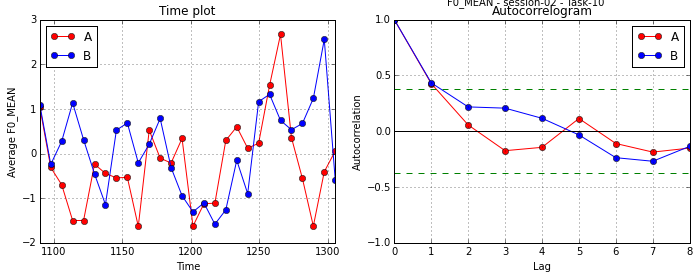
\includegraphics[width=15cm]{images/time_plot_with_autocorrelation.png}
\caption{Time-plot generado por el método TAMA, junto a su autocorrelograma}
\label{fig:time_plot}
\end{figure}

El hecho de que los autocorrelogramas desciendan rápidamente a cero es un indicio de que las series de tiempo construidas son estacionarias, como se menciona en la Sección \ref{sec:autocorrelation}. Esto nos habilita a efectuar el análisis bivariado de las series.

\section{Medición del Entrainment}
\label{sec:method_entrainment}

Considerando todo lo mencionado, procedimos a definir una medida de \entrainment basándonos en el cálculo de la correlación cruzada muestral. Recordemos que, bajo la definición dada en la ecuación \ref{cross_correlation_definition} de $r_{AB}(k)$, al tomar $k \geq 0$ medíamos cuánto influía $B$ sobre los futuros valores de $A$, y viceversa cuando $k \leq 0$. Se tomó la decisión de que este cálculo sólo se realice cuando el desplazamiento resulta en al menos 4 puntos que se solapan; si esto no ocurre, dejamos indefinido el valor en el correlograma cruzado.

Con esto en mente, definimos una primer métrica $\fwentrainment{AB}^{(1)}$ como el valor de $r_{AB}(k)$ con mayor valor absoluto, dado $k \leq 0$. Análogamente lo definimos para $\fwentrainment{BA}^{(1)}$.

En segundo lugar, definimos una segunda métrica $\fwentrainment{BA}^{(2)}$, como el valor absoluto de la primera, es decir:

\begin{equation}
\fwentrainment{BA}^{(2)} = |\fwentrainment{BA}^{(1)}|
\end{equation}

Por último, cabe mencionar que a diferencia de \cite{KOU2008.2} dónde sólo se hacía un análisis de significancia, nosotros vamos a utilizar esta medida independientemente de si es o no estadísticamente diferente de cero.

\section{Panel de datos}
\label{sec:panel_data}

Luego de construir las series de tiempo para cada una de las conversaciones que seleccionamos anteriormente, pasamos a construir una gran tabla que se utilizó en los experimentos de regresión detallados en la siguiente sección. Para condensar todos nuestros datos, armamos una tabla por cada variable acústico-prosódicas, que contiene información definida para cada interlocutor y tarea de nuestro corpus.

Cada columna de esta tabla representa los datos de un interlocutor dentro de una tarea. Éste hecho lo usamos fuertemente a la hora de definir los grupos en nuestro modelo de Efectos Fijos. En la figura \ref{fig:panel_data} se describen las columnas generadas.

\begin{figure}[b!]
\centering
\adjustbox{max width=\textwidth}{
\begin{tabular}{|c|c|}
  \hline
  \myhighlight \emph{Campo} & \emph{Descripción} \\\hline
  session & número de sesión \\\hline
  speaker & 0 si corresponde al interlocutor A; B en otro caso \\\hline
  task & número de tarea \\\hline
  count & La cantidad de puntos definidos que tiene la serie \\\hline
  entrainment & Si $speaker=0$, es $\fwentrainment{AB}$; $\fwentrainment{BA}$ en otro caso \\\hline
  best\_lag & el lag del cross-correlogram donde se logra el \emph{entrainment} \\\hline

  engaged\_in\_game & ¿el sujeto parece comprometido con el juego? \\\hline
  difficult\_for\_partner\_to\_speak & ¿el sujeto dirige la conversación? \\\hline
  contributes\_to\_successful\_completion & ¿el sujeto contribuye para el éxito del equipo? \\\hline
  gives\_encouragement & ¿el sujeto alienta a su compañero?\\\hline
  making\_self\_clear & ¿el sujeto se expresa correctamente?\\\hline

  planning\_what\_to\_say & \\\hline
  bored\_with\_game & ¿el sujeto se muestra aburrido? \\\hline
  dislikes\_partner &  ¿al sujeto no le agrada su compañero? \\\hline
\end{tabular}}
\label{fig:panel_data}
\caption{Columnas de la tabla generada para ser utilizada en los experimentos de regresión lineal}
\end{figure}



La tabla generada tuvo una dimensión de 210 x 21, siendo 210 la cantidad de tareas (contadas dos veces por cada hablante) y 21 las columnas mencionadas en la figura \ref{fig:panel_data}. Una forma de ver ésta tabla es que, para cada sesión y hablante, tenemos una serie de tiempo sobre las tareas   siendo los datos el entrainment y las variables sociales. En la jerga econométrica, llamamos a este tipo de datos \emph{de panel}\cite{gujarati1999}: un conjunto de mediciones temporales sobre un mismo sujeto a lo largo del tiempo. En este caso el sujeto es un interlocutor en una sesión, el tiempo son las tareas, y las mediciones son los entrainments y las diferentes variables sociales.

En la figura \ref{fig:panel_data_example} tenemos una sección de la tabla. Los sujetos que tenemos en éste ejemplo son 3: $speaker = 0$ y $session=1$, $speaker = 1$ y $session=1$, y $speaker = 0$ y $session=2$. También tenemos cinco series de tiempo para cada sujeto: \entrainment, \emph{bored}, \emph{engaged}, \emph{encourages} y \emph{clear}. Vale la pena remarcar que estas series de tiempo, al igual que las que consideramos en la construcción de TAMA, pueden tener datos faltantes.


\begin{figure}
\centering
\adjustbox{max width=\textwidth}{
\begin{tabular}{lrrrrrrrrr}
\toprule
session &  speaker &  task &  entrainment &  bored\_with\_game &  engaged\_in\_game &  gives\_encouragement &  making\_self\_clear &  planning\_what\_to\_say \\
\midrule
1 &        0 &    10 &     0.581475 &                0 &                5 &                    5 &                  5\\
1 &        0 &    12 &    -0.569677 &                1 &                5 &                    5 &                  5\\
1 &        0 &    13 &     0.533701 &                2 &                4 &                    5 &                  4\\
1 &        1 &    10 &    -0.917101 &                0 &                5 &                    2 &                  3\\
1 &        1 &    12 &     0.467112 &                0 &                5 &                    4 &                  2\\
1 &        1 &    13 &    -0.602364 &                0 &                5 &                    4 &                  3\\
2 &        0 &     3 &     0.520696 &                0 &                4 &                    5 &                  5\\
2 &        0 &     4 &    -0.241060 &                0 &                5 &                    4 &                  4\\
2 &        0 &     7 &     0.743719 &                0 &                5 &                    4 &                  5\\
2 &        0 &     8 &     0.147362 &                0 &                5 &                    4 &                  2\\
\bottomrule
\end{tabular}
}


\caption{Ejemplo de tabla generada para $\FOMEAN$}
\label{fig:panel_data_example}
\end{figure}


\begin{figure}
\centering
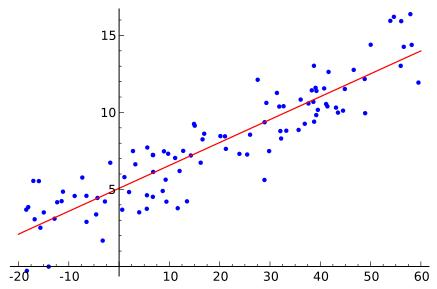
\includegraphics[width=10cm]{images/linear_regression.jpg}
\caption{Ejemplo de Regresión Lineal}
\end{figure}

\section{Análisis de regresión}

Llegado a este punto, dada una variable a/p, nos interesaría evaluar la relación entre el entrainment y las distintas variables sociales. Con esto en mente, planteamos un modelo de regresión lineal donde nuestra variable explicativa será la mimetización, y la variable \emph{dependiente} será la variable social.

En base a ésto, podremos observar cuál es la variación conjunta de ellas. Es esperable que, al aumentar la mimetización, aumenten ciertas variables sociales (por ejemplo, la compenetración en el juego) y que otras desciendan (el aburrimiento).


\subsection{Modelo clásico de Regresión Lineal}

En el modelo clásico de regresión lineal, tenemos un conjunto de valores fijos $X_1, X_2, \ldots, X_n$, que son llamadas variables independientes. Asociado a cada uno de estos valores fijos, tenemos variables aleatorias $Y_1, \ldots, Y_n$. Asumimos, además, que nuestras variables son de la forma

\begin{equation}
  Y_i = E[Y|X_i] + u_i
\end{equation}

donde $u_i$ es la perturbación estocástica de la variable.

Asumiendo que $E[Y|X_i]$ es una función lineal de $X_i$; es decir, que existen $\beta_1, \beta_2 \in \mathbb{R}$ que cumplen

\begin{equation}
  E[Y|X_i] = \beta_1 + \beta_2 X_i
\end{equation}

obtenemos que

\begin{equation}
  Y_i = \beta_1 + \beta_2 X_i + u_i
\end{equation}

Nuestro objetivo es poder entonces conseguir estimadores $\widehat{\beta_1}, \widehat{\beta_2}$ que nos permitan analizar y predecir el comportamiento conjunto de estas variables.

\subsection{Nuestro modelo}

Sea entonces una variable acústica/prosódica (por ejemplo, el pitch o la intensidad), y una variable social de las que acabamos de enumerar en \ref{sec:panel_data}. Sean $E_1, \ldots, E_n$ los valores de entrainment para el set de datos que definimos en \ref{sec:panel_data}, y sean $V_1, V_2, \ldots V_n$ los valores de la variable social de cada conversación.

Sobre éstas variables es que planteamos nuestro modelo de regresión lineal clásica: queremos ver qué relación hay tomando como variable ``fija'' al entrainment, y como variable dependiente a la variable social. Queremos hallar, entonces $\widehat{\beta_1}, \widehat{\beta_2} \in \mathbb{R}$

\begin{equation}
  V_i \simeq \widehat{\beta_1} + \widehat{\beta_2} E_i
\end{equation}


Para ello, calcularemos los estimadores $\widehat{\beta_1}, \widehat{\beta_2} \in \mathbb{R}$ mediante el método \emph{QR} (insertar referencia aquí) que nos provee el lenguaje R. A su vez, luego de ésto efectuaremos un análisis de significancia sobre $\beta_2$ para verificar que sean distintos de 0.


Uno esperaría que un alto \emph{entrainment} se relacione con un alto valor de ciertas variables sociales \cite{BRE1996}, por ejemplo la compenetración con el juego, el ayudar a terminarlo. Esto significa esperar que el valor de $\widehat{\beta_2}$; y se relacione con bajos valores de otras, como el aburrimiento, o el rechazo percibido hacia el compañero.







\section{Resultados}
\begin{frame}
\frametitle{Resultados de Regresión Agrupada}

  Regresión Agrupada: Hacemos regresión lineal sobre todos los datos, independientemente de su origen.

  \begin{enumerate}
    \item Para $\fwentrainment{AB}^{(1)}$ no hubo casi resultados significativos
    \item Para $\fwentrainment{AB}^{(2)}$ hubo resultados significativos, pero pocos
  \end{enumerate}

  Para analizar mejor los resultados y eliminar las variables no medidas, efectuamos un análisis de Efectos Fijos.
\end{frame}

\begin{frame}
\frametitle{Regresión Lineal con Efectos Fijos}

  \begin{columns}
    \column{0.40\textwidth}
    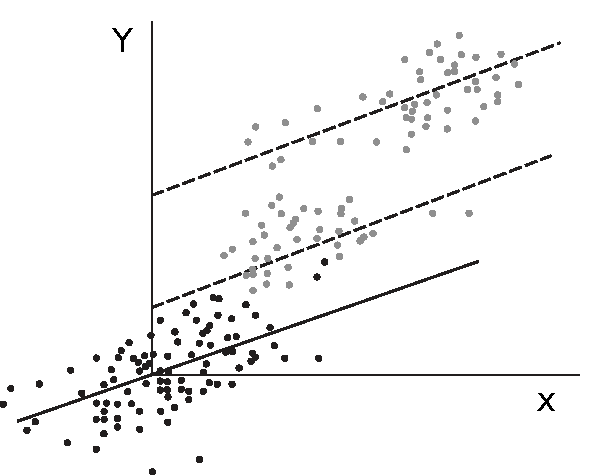
\includegraphics[width=\textwidth]{images/fixed_effects_example.pdf}
    \column{0.60\textwidth}
    \begin{itemize}
      \item Modelo agrupado: niega la posibilidad de heterogeneidad por cada sujeto
      \item Modelo efectos fijos: heterogeneidad no observada constante en el tiempo para cada sujeto.
      \item Varias formas equivalentes de calcularlo: Dummy Variable, Within Group.
      \item En nuestro caso: un sujeto es un hablante dentro de una sesión particular.
    \end{itemize}
  \end{columns}
\end{frame}


\begin{frame}
\frametitle{Regresión Lineal con Efectos Fijos}
\framesubtitle{Resultados}

\begin{table}
  \begin{figure}[ht]
\centering
% psl is "Positive Slope"
\newcommand{\psl} { $+$ }
% nsl stands for "Negative SLope"
\newcommand{\nsl} { $-$ }


\begin{tabular}{| c | c | c | c | c | c |}
  \hline
 & ENG\_MAX & ENG\_MEAN & F0\_MEAN & F0\_MAX & NOISERATIO  \\
  \hline
contributes  &      &  & \psl &  & \psl \\ \hline
  clear     & \psl &  & \psl &  & \psl \\ \hline
  engaged    &      &  & \psl &  &      \\ \hline
  planning   &      &  &      &  &      \\ \hline
  encourages &      &  &      &  &      \\ \hline
  difficult  & \nsl &  &      &  &      \\ \hline
  bored      &      &  & \nsl &  &      \\ \hline
  dislikes   &      &  &      &  &      \\ \hline
   \hline
\end{tabular}

\adjustbox{max width=\textwidth}{
\begin{tabular}{| c | c | c | c | c | c | c |}
  \hline
& PHON\_AVG & PHON\_COUNT & SHIMMER & SYL\_AVG & SYL\_COUNT & VCD2TOT \\
  \hline
contributes  &      &  &  &  &      &  \\ \hline
  clear     & \psl &  &  &  & \psl &  \\ \hline
  engaged    &      &  &  &  &      &  \\ \hline
  planning   &      &  &  &  &      &  \\ \hline
  encourages &      &  &  &  &      &  \\ \hline
  difficult  &      &  &  &  &      &  \\ \hline
  bored      &      &  &  &  &      &  \\ \hline
  dislikes   &      &  &  &  &      &  \\ \hline
  \hline
\end{tabular}
}

\caption{Tabla que representa los resultados significantes del experimento. En una de las entradas, tenemos los nombres abreviados de las variables sociales, y en la otra las variables a/p. El símbolo \psl representa valor significante y positivo de la pendiente de la regresión de efectos fijos, mientras que \nsl representa significante y negativo }

\label{sign_table}

\end{figure}

\end{table}

Tabla que resume los resultados significativos del análisis con efectos fijos. \psl indica un valor positivo con significancia $p < 0.10$,  \ppsl con $p < 0.05$  y \pppsl con $p < 0.01$. Análogamente para los valores negativos.

\end{frame}


\begin{frame}
\frametitle{Regresión Lineal con Efectos Fijos}
\framesubtitle{Resultados}
\begin{enumerate}
  \item Casi todas las variables \ap poseen al menos un valor significativo de $\estslope$, destacándose \ENGMEAN, \NOISETOHARMONICS y \FOMEAN.
  \item Las variables sociales positivas se relacionan de manera positiva con la métrica de mimetización, en aquellos casos significantes.
  \item Análogamente ocurre con las variables de connotación negativa, aunque de manera menos clara.
  \item La métrica se comporta de manera consistente a medidas de mimetización acústico-prosódicas desarrolladas en otros trabajos, como en Gravano et al (2015) utilizando patrones entonacionales. \footnote{Agustin Gravano, Stefan Benus, Rivka Levitan, and Julia Hirschberg. Backward mimicry and forward influence in prosodic contour choice in standard american english 2015.}
\end{enumerate}
\end{frame}


\section{Conclusiones}
En el presente trabajo, analizamos como dos métricas del \entrainment derivadas automáticamente de la conversación se relacionan con la percepciones sociales de terceros independientes del juego. Todo este análisis se da en el contexto de un juego orientado a tareas, que comprende interacciones de una naturaleza muy similar a las de una interfaz humano-computadora.

Estas métricas fueron construídas a través del análisis de series de tiempo, y apuntan a cuantificar cuánto se imitan o mimetizan los hablantes en términos de sus variables acústico-prosódicas. En primer lugar, contemplamos una métrica que penaliza el dis-entrainment con valores negativos. Se aplicó análisis de regresión sobre esta métrica, y los resultados que dio no fueron significativos. En segundo lugar, construimos una métrica que valora de igual manera el \entrainment y el dis-\entrainment, de acuerdo a literatura que sugería que el segundo fenómeno puede considerarse en algunas circunstancias como un mecanismo de adaptación cooperativa. Al efectuar el análisis de regresión sobre ésta, los resultados fueron significativos y consistentes a la hipotesis planteada de que el \entrainment se relaciona positivamente con características sociales favorables de la conversación, mientras que lo hace de manera inversa con aquellas negativas.

Respecto a trabajos anteriores donde se construyen medidas del \entrainment prosódico, la métrica construída se comporta de manera consistente, manteniendo las relaciones entre aquellas variables sociales de carácter positivo y negativo. Esta métrica, además, se puede efectuar sin intervención manual a diferencia de aquellas que utilizan ToBI o anotaciones de otro tipo. A su vez, la cuantificación presentada evita el problema del alineamiento de turnos mediante la abstracción de éstos usando series de tiempo.

Una contribución importante de este trabajo es la validación de la métrica introducida en \cite{KOU2008.2}, dando indicios de que ésta guarda relación con la percepción social de la conversación. Igual de importante es el uso del valor absoluto de la correlación cruzada, como medida unificadora del \entrainment y \disentrainment y que remarca la importancia deĺ segundo fenómeno dentro de la comunicación verbal, a la luz de últimos trabajos acerca de la divergencia en el diálogo.

A pesar de que los resultados son prometedores, siguen siendo preliminares y la robustez de estos requieren más validaciones. Como trabajo a futuro, proponemos reproducir estos experimentos sobre otros corpus de habla. Adicionalmente, se debería verificar el impacto del proceso de pre-whitening, ya que un análisis a priori no mostró grandes diferencias entre usar o no este filtro. Otra dirección posible es evaluar un análisis multivariado de las diferentes variables \ap para construir una medida del \entrainment prosódico.


\end{document}
